
%(BEGIN_QUESTION)
% Copyright 2011, Tony R. Kuphaldt, released under the Creative Commons Attribution License (v 1.0)
% This means you may do almost anything with this work of mine, so long as you give me proper credit

Følgende temperaturreguleringssystem er hel-pneumatisk, med pneumatisk transmitter, regulator og luft-til-stenge reguleringsventil. Oppgaven din er å skissere nødvendige rør- og ledningsforbindelser slik at reguleringsventilen går til sin ``fail-safe''-posisjon når en operatør trykker på trykknappen:

$$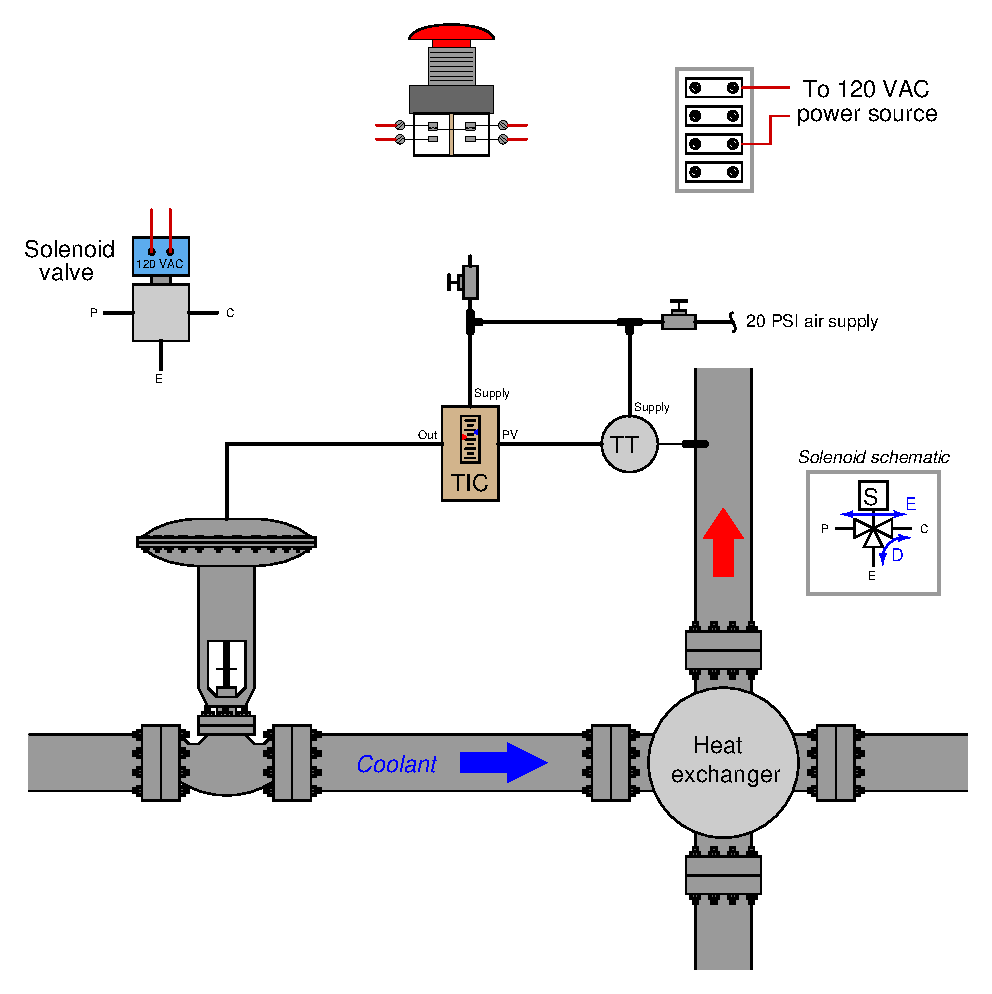
\includegraphics[width=15.5cm]{i01447x01.eps}$$

Systemet er nå tegnet uten at avstengingssolenoiden er koblet i det hele tatt. Du kan gjerne ``bryte'' og rute om eksisterende rør etter behov for å modifisere systemet slik at det inkluderer magnetventilen, og at regulatorens utgangssignal bypasses når knappen trykkes.
 
\underbar{file i01447}
%(END_QUESTION)





%(BEGIN_ANSWER)

Alt må være riktig i diagrammet for å få uttelling: bryteren må bruke sin NC-kontakt (de-energiseres når knappen trykkes), med ventilrøret koblet til ``C'', regulatoren til ``P'', og ``E'' ventilert:

$$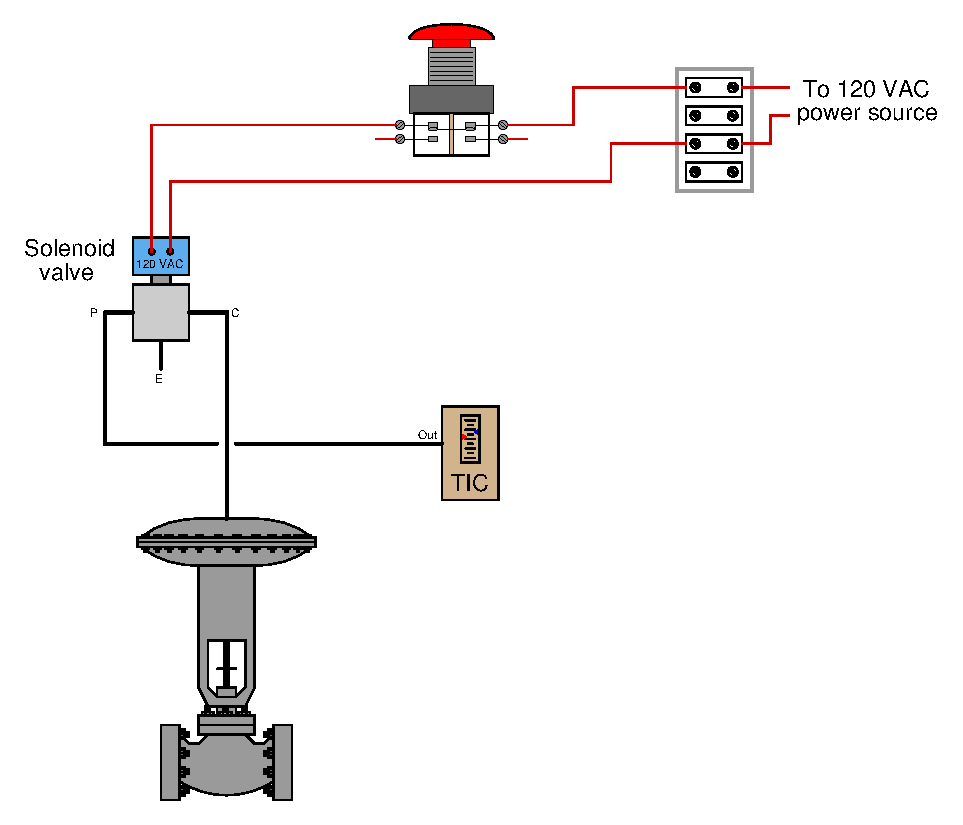
\includegraphics[width=15.5cm]{i01447x02.eps}$$

En alternativ løsning der magnetventilen stopper og ventilerer luft fra regulatorens forsyningsrør fungerer like bra, og gir full uttelling.

En alternativ metode der ``P'' ventileres og ``E'' går til regulatoren vil også fungere dersom bryteren er koblet NO. Denne løsningen bør imidlertid bare gis 8 poeng, ikke full pott (fordi dette ikke er standard bruk av P-, C- og E-portene på en 3-veis ventil).

Hvis en student foreslår en løsning som ville ventilere luft fra ventilen, men bare ved å lufte forsyningstrykket direkte til atmosfæren, gi kun halv uttelling (5 poeng). En slik løsning vil riktignok få ventilen til å gå til fail-posisjon, men den er svært upraktisk og sløsende med instrumentluft.

%(END_ANSWER)





%(BEGIN_NOTES)

{\bf Dette spørsmålet er ment for eksamen og ikke arbeidsark!}.

%(END_NOTES)

